\documentclass[10pt]{article}
\usepackage{amsmath}
\usepackage{listings}
\usepackage{textcomp}
\usepackage{graphicx}
\usepackage[utf8]{inputenc} % allow utf-8 input
\usepackage[T1]{fontenc}    % use 8-bit T1 fonts
\usepackage{hyperref}       % hyperlinks
\usepackage{url}            % simple URL typesetting
\usepackage{booktabs}       % professional-quality tables
\usepackage{amsfonts}       % blackboard math symbols
\usepackage{nicefrac}       % compact symbols for 1/2, etc.
\usepackage{microtype}      % microtypography
\setlength{\parindent}{0pt}

\graphicspath{{../}}

\newcommand{\skipline}{\vspace{\baselineskip}}

\begin{document}

\normalsize

\begin{abstract}
	\quad We implement a naive multi-layer perceptron model that trained on amount of 10 games to solve the agent modeling problem of the ad-hoc challenge. The data we generate from script has 150 games. We performed a 15-fold; 10 random games are chosen as training set and remaining as validation set for each fold, so that training sets across all folds are mutually exclusive. For hyper-parameter optimization, we used random search on around 8,500 sets of hyper-parameters, seeking a model that give us the best accuracy.
\end{abstract}

\section{Approach}
	\quad We first provide code for formatting the data into training and validation data. After formatting, an input is a 658 bit binary vector representing the observation an agent sees in a round and an output is a one-hot encoded vector with a length of 20 representing the action that the agent takes, so the size of the input and output layer can be determined already. We have several hyper-parameters to adjust in our model. Specifically, we have hidden layer sizes, number of neurons in hidden layer, activation function for each hidden layer, learning rate, batch size, and options for batch normalization, dropout, and regularization. We performed random hyper-parameter search [1] by generating 8,500 random parameter combinations for our model to observe the change in accuracy on validation data. Most of these hyper-parameters are chosen uniformly randomly except for choosing Batch Normalization and Dropout, where we prevented them from being used at the same time. The reason of this is that Batch Normalization and Dropout can negatively affect each other and bring down the performance of the model as shown in [2] by Li \textit{et al}. To reduce computation time, we made the assumption \footnote{In the actual code, fold number starts from 0 and approximation uses agents 1 \& 6, but here in the formula, fold number starts from 1 and approximation uses agents 1 \& 2 for demonstration purpose. The reason that agents 1 \& 6 are chosen is that we noticed models for agent 1 perform below average while models for agent 6 perform above.}

  \begin{align*}
    Mean Acc &=
    \frac{1}{\lVert agents\rVert*\lVert folds\rVert}\sum_{i=1}^{\lVert agents\rVert}\sum_{j=1}^{\lVert folds\rVert} \frac{count(\hat{Y}_{ij}=Y_{ij})}{\lVert Y_{ij} \rVert}\\
    &\approx
    \frac{1}{2}
    \sum_{i=1}^{2}\sum_{j=1}^{1} \frac{count(\hat{Y}_{ij}=Y_{ij})}{\lVert Y_{ij} \rVert}
  \end{align*}


  where $count(\hat{Y}_{ij}=Y_{ij})$ denotes the number of elements in prediction vector $\hat{Y}$ matching the corresponding elements in the true value vector $Y$; thus, only 2 models are computed to calculate the average 15-fold validation accuracy for each set of hyper-parameters instead of $6 * 15$ models. We also ran multiple sets of hyperparameters on CSIF machines in parallel to further increase the efficiency.

  \quad Inside our \texttt{hyper\_search.py}, we provide all the significant hyper parameters, with default range of learning rate from 0 to 1, number of hidden layers from 1 to 3, number of neurons from 25 to 500, learning rate decay from 0 to 0.01, and possible activation functions being LeakyReLU, ReLU, ELU, PReLU. These ranges are shrinked manually as we continue searching for more sets.

\section{Results}

  \begin{center}
    \textit{Top Three Sets of Hyper-parameters with Approximated Mean Fold Acc.}
    \scriptsize
    \begin{tabular}{| c | c | c | c | c | c | c | c | c | c |}
      \hline
      Set & Acc & LR & BS & Act. & Hidden & Decay & BNorm & Dropout & Reg \\
      \hline
      1 & 0.44428  &  0.00034 & 44 & ReLU  & 366-139 & 0.00037 & False & True & None \\
      2 & 0.44352  &  0.00151 & 35 & PReLU & 214     & 0.00055 & False & True & None \\
      3 & 0.44227  &  0.00015 & 32 & PReLU & 463     & 0.00032 & False & True & None \\
      \hline
    \end{tabular}
    \normalsize
  \end{center}

  \quad The accuracies above are calculated with the approximation based on the assumption from the previous page. These hyperparameters were then run on all of the six agents and 15 folds. The results are below.

  \begin{center}

    \textit{Set 1}

    \textit{Total Avg Acc: 0.42997}
    \footnotesize
    \begin{tabular}{| c | c | c | c | c | c | c |}
      \hline
       & agent 1 & agent 2 & agent 3 & gent 4 & agent 5 & agent 6 \\
      \hline
      fold 0 & 0.42 & 0.48 & 0.40 &  0.42 &  0.38 & 0.46 \\
      fold 1 & 0.41 & 0.49 & 0.41 &  0.42 &  0.39 & 0.46 \\
      fold 2 & 0.41 & 0.49 & 0.42 &  0.41 &  0.37 & 0.48 \\
      fold 3 & 0.42 & 0.47 & 0.42 &  0.42 &  0.38 & 0.46 \\
      fold 4 & 0.40 & 0.46 & 0.42 &  0.42 &  0.38 & 0.47 \\
      fold 5 & 0.41 & 0.49 & 0.43 &  0.42 &  0.38 & 0.46 \\
      fold 6 & 0.40 & 0.48 & 0.41 &  0.42 &  0.40 & 0.46 \\
      fold 7 & 0.42 & 0.48 & 0.42 &  0.43 &  0.38 & 0.47 \\
      fold 8 & 0.42 & 0.49 & 0.40 &  0.42 &  0.38 & 0.47 \\
      fold 9 & 0.41 & 0.47 & 0.42 &  0.41 &  0.36 & 0.46 \\
      fold 10 & 0.42 & 0.46 & 0.42 &  0.43 &  0.38 & 0.48 \\
      fold 11 & 0.40 & 0.47 & 0.40 &  0.41 &  0.38 & 0.48 \\
      fold 12 & 0.42 & 0.47 & 0.43 &  0.43 &  0.38 & 0.50 \\
      fold 13 & 0.41 & 0.48 & 0.42 &  0.43 &  0.37 & 0.46 \\
      fold 14 & 0.40 & 0.48 & 0.44 &  0.42 &  0.39 & 0.46 \\
      Avg  & 0.411 & 0.477 & 0.417 &  0.422 &  0.382 & 0.469 \\
      \hline
    \end{tabular}
    \normalsize

    \newpage

    \textit{Set 2}

    \textit{Total Avg Acc: 0.42979}
    \footnotesize
    \begin{tabular}{| c | c | c | c | c | c | c |}
      \hline
       & agent 1 & agent 2 & agent 3 & gent 4 & agent 5 & agent 6 \\
      \hline
      fold 0 & 0.42 & 0.49 & 0.40 & 0.42 & 0.38 & 0.45 \\
      fold 1 & 0.42 & 0.49 & 0.41 & 0.42 & 0.40 & 0.46 \\
      fold 2 & 0.41 & 0.49 & 0.43 & 0.42 & 0.38 & 0.48 \\
      fold 3 & 0.42 & 0.48 & 0.43 & 0.42 & 0.38 & 0.47 \\
      fold 4 & 0.40 & 0.46 & 0.42 & 0.43 & 0.38 & 0.47 \\
      fold 5 & 0.41 & 0.49 & 0.43 & 0.42 & 0.38 & 0.45 \\
      fold 6 & 0.40 & 0.48 & 0.41 & 0.42 & 0.40 & 0.47 \\
      fold 7 & 0.42 & 0.49 & 0.42 & 0.43 & 0.37 & 0.47 \\
      fold 8 & 0.42 & 0.49 & 0.41 & 0.42 & 0.37 & 0.47 \\
      fold 9 & 0.41 & 0.47 & 0.41 & 0.42 & 0.35 & 0.46 \\
      fold 10 & 0.41 & 0.46 & 0.42 & 0.43 & 0.38 & 0.47 \\
      fold 11 & 0.40 & 0.47 & 0.40 & 0.42 & 0.38 & 0.48 \\
      fold 12 & 0.41 & 0.47 & 0.44 & 0.43 & 0.39 & 0.50 \\
      fold 13 & 0.41 & 0.49 & 0.42 & 0.42 & 0.37 & 0.45 \\
      fold 14 & 0.40 & 0.48 & 0.43 & 0.42 & 0.39 & 0.47 \\
      Avg & 0.410 & 0.479 & 0.417 & 0.422 & 0.382 & 0.469 \\
      \hline
    \end{tabular}
    \normalsize

    \skipline

    \textit{Set 3}

    \textit{Total Avg Acc: 0.43002}
    \footnotesize
    \begin{tabular}{| c | c | c | c | c | c | c |}
      \hline
       & agent 1 & agent 2 & agent 3 & gent 4 & agent 5 & agent 6 \\
      \hline
      fold 0 & 0.42 & 0.49 & 0.40 & 0.42 & 0.38 & 0.45 \\
      fold 1 & 0.42 & 0.49 & 0.41 & 0.42 & 0.40 & 0.46 \\
      fold 2 & 0.41 & 0.49 & 0.43 & 0.42 & 0.38 & 0.48 \\
      fold 3 & 0.42 & 0.48 & 0.43 & 0.42 & 0.38 & 0.47 \\
      fold 4 & 0.40 & 0.46 & 0.42 & 0.43 & 0.38 & 0.47 \\
      fold 5 & 0.41 & 0.49 & 0.43 & 0.42 & 0.38 & 0.45 \\
      fold 6 & 0.40 & 0.48 & 0.41 & 0.42 & 0.40 & 0.47 \\
      fold 7 & 0.42 & 0.49 & 0.42 & 0.43 & 0.37 & 0.47 \\
      fold 8 & 0.42 & 0.49 & 0.41 & 0.42 & 0.37 & 0.47 \\
      fold 9 & 0.41 & 0.47 & 0.41 & 0.42 & 0.35 & 0.46 \\
      fold 10 & 0.41 & 0.46 & 0.42 & 0.43 & 0.38 & 0.47 \\
      fold 11 & 0.40 & 0.47 & 0.40 & 0.42 & 0.38 & 0.48 \\
      fold 12 & 0.41 & 0.47 & 0.44 & 0.43 & 0.39 & 0.50 \\
      fold 13 & 0.41 & 0.49 & 0.42 & 0.42 & 0.37 & 0.45 \\
      fold 14 & 0.40 & 0.48 & 0.43 & 0.42 & 0.39 & 0.47 \\
      Avg & 0.410 & 0.479 & 0.417 & 0.422 & 0.382 & 0.469 \\
      \hline
    \end{tabular}
    \normalsize
  \end{center}

  \quad Although the difference is negligible, set 3 achieves the best accuracy and will be used as the hyper-parameters for our final model. An overview of the model is below.

  \newpage
  \begin{center}
    \textit{Model Overview}

    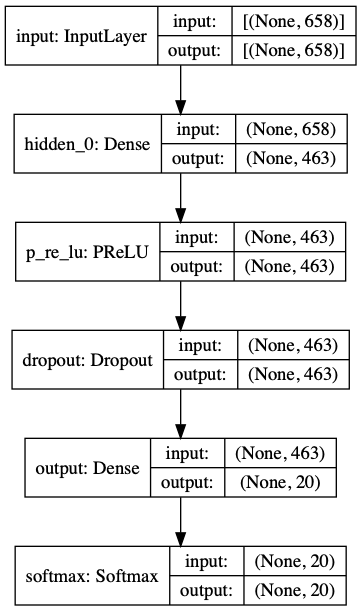
\includegraphics[width=0.4\textwidth]{best_model.png}
  \end{center}

  \quad Since the hyper-parameters are chosen with the validation sets, we generated a new dataset with 100 games as our final validation set for our model. The results from running 10-fold cross validation on this dataset with hyper-parameter set 3 are below.

  \begin{center}
    \textit{Set 3 on Final Testing Set}

    \textit{Total Avg Acc: 0.42382}
    \footnotesize
    \begin{tabular}{| c | c | c | c | c | c | c |}
      \hline
       & agent 1 & agent 2 & agent 3 & gent 4 & agent 5 & agent 6 \\
      \hline
      fold 0 & 0.40 & 0.48 & 0.41 & 0.42 & 0.37 & 0.46 \\
      fold 1 & 0.41 & 0.47 & 0.39 & 0.41 & 0.37 & 0.44 \\
      fold 2 & 0.40 & 0.49 & 0.40 & 0.41 & 0.38 & 0.46 \\
      fold 3 & 0.40 & 0.46 & 0.39 & 0.43 & 0.38 & 0.50 \\
      fold 4 & 0.40 & 0.48 & 0.41 & 0.43 & 0.38 & 0.43 \\
      fold 5 & 0.41 & 0.47 & 0.41 & 0.42 & 0.37 & 0.45 \\
      fold 6 & 0.42 & 0.48 & 0.38 & 0.43 & 0.37 & 0.49 \\
      fold 7 & 0.40 & 0.49 & 0.41 & 0.43 & 0.39 & 0.43 \\
      fold 8 & 0.42 & 0.49 & 0.40 & 0.43 & 0.38 & 0.45 \\
      fold 9 & 0.41 & 0.47 & 0.40 & 0.44 & 0.35 & 0.46 \\
      Avg & 0.408 & 0.477 & 0.401 & 0.426 & 0.374 & 0.457 \\
      \hline
    \end{tabular}
    \normalsize
  \end{center}

  \quad One might think that an accuracy of 0.42 is quite high because there are 20 classes which means guessing randomly should only achieve an accuracy of 0.05; however, this is based on the assumption that the distribution of the classes is uniformly random which is unfortunately not the case here as shown in the histograms below.


  \newpage
  \begin{center}
    \textit{Action Distribution for the Tuning Dataset with 150 Games.}

    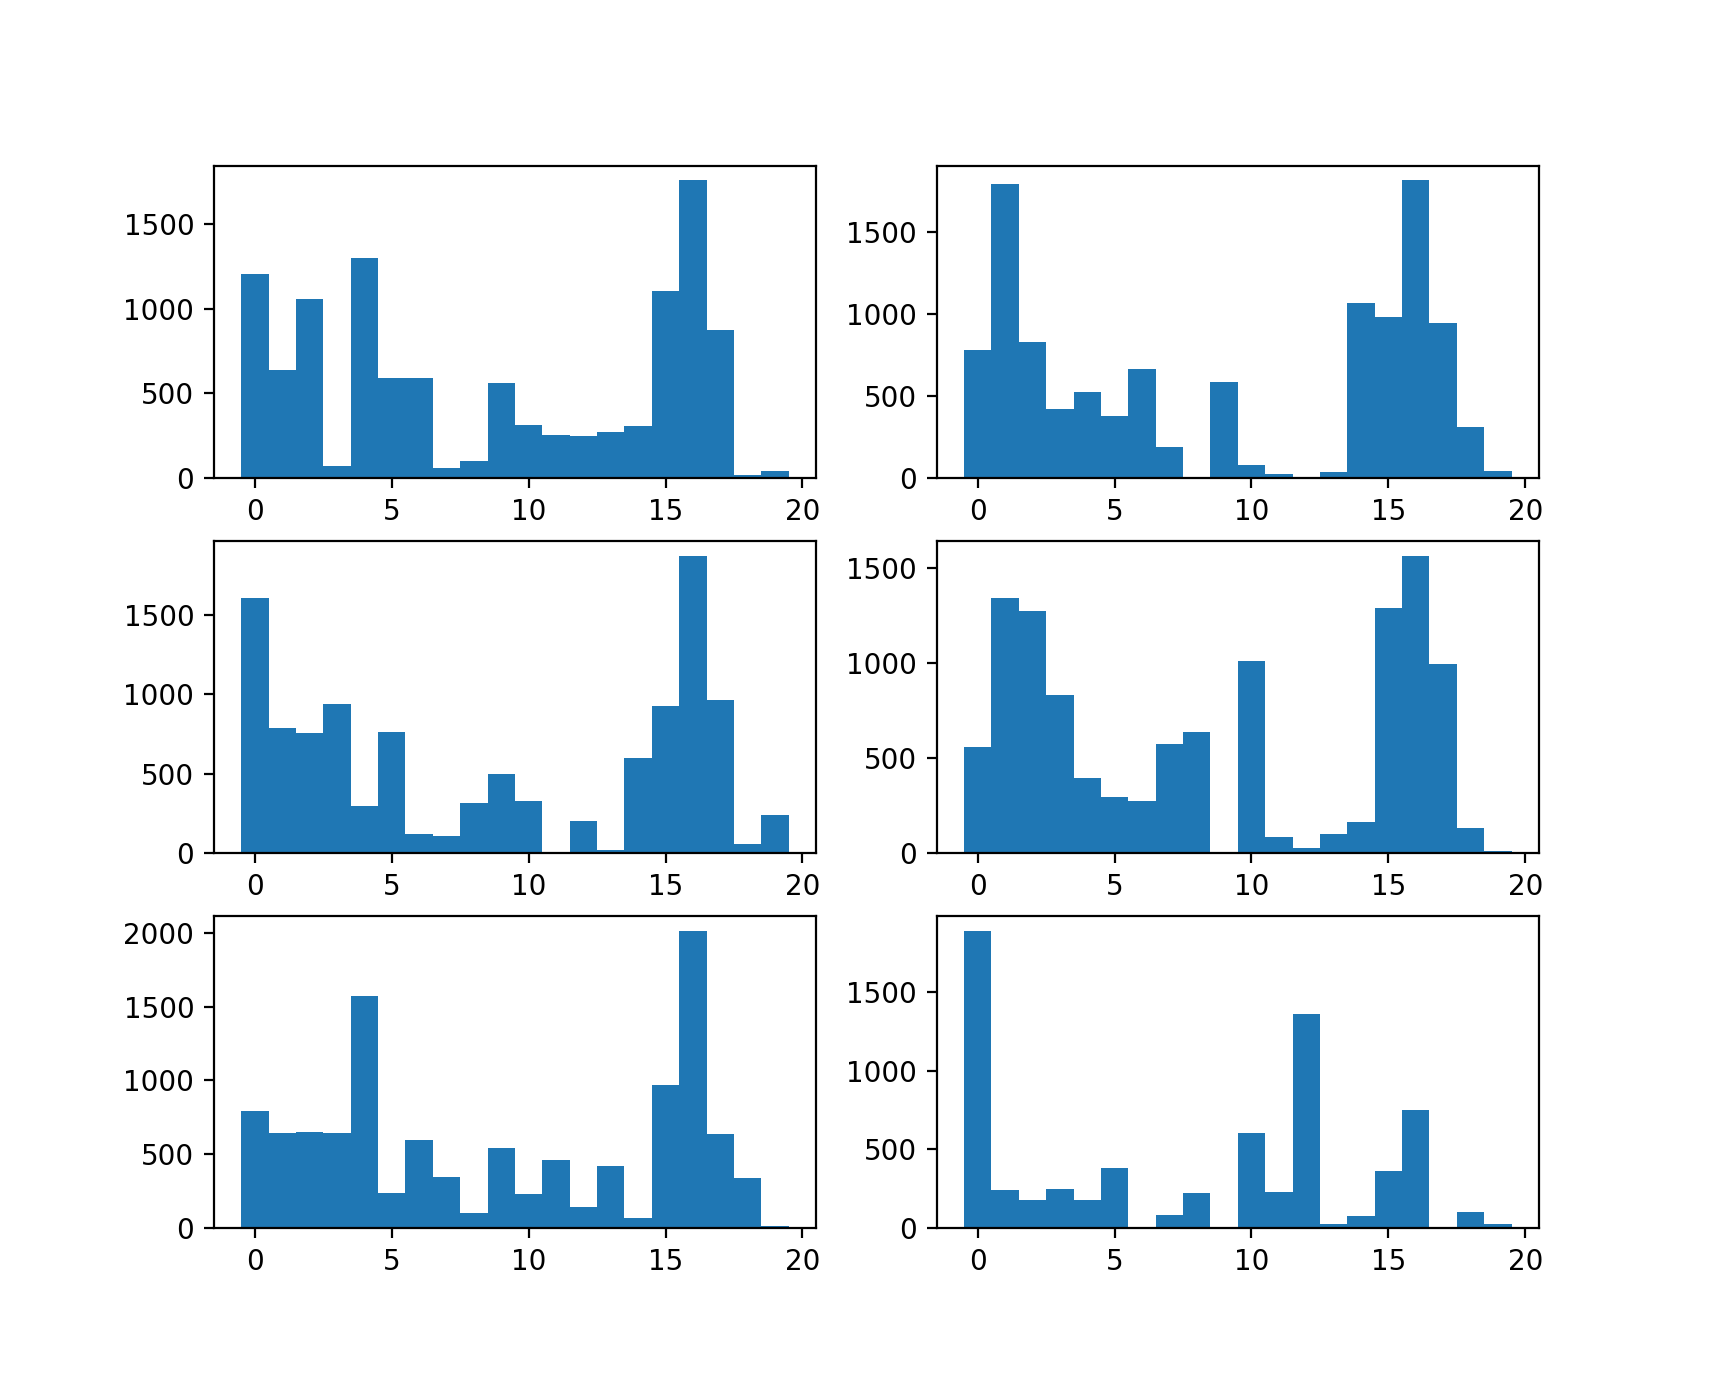
\includegraphics[width=0.8\textwidth]{agent1-6_action_dist.png}

    \scriptsize

    \textit{Note: The plots correspond to agent 1 to 6 in the order of left to right and top to bottom.}

    \normalsize
  \end{center}

  \quad For instance, although the models achieve an accuracy of around 0.45 on predicting agent 6's action, it becomes less appealing when a model that simply only guesses action 0 can achieve an accuracy of around 0.35.

\section{Possible Improvements}

  \quad One possible improvement is to plot out PR curves and try to tackle the unbalanced dataset problem with oversampling techniques, such as ADASYN [3]. However, this can be challenging since certain actions have never been performed by an agent, so it is very difficult, if not impossible, to oversample these classes.

  \quad Another possible improvement is to investigate the reason that the model performs significantly worse on predicting agent 5's action than other agents. Simply based on the histograms, distribution of agent 5's actions do not seem to be much different from agent 1 to 4, which removes the possibility that agent 5 has a different bias towards the actions from other agents. Thus, one of the most pausible explanations that's left is that agent 5 simply responds to observations differently than the others. If a pattern can be found in agent 5's response to observations, then it will be possible to improve the model's accuracy on predicting agent 5 and thus improve the overall accuracy.

\skipline

\newpage \section*{References}

\footnotesize

  [1]	James Bergstra, Yoshua Bengio. Random Search for Hyper-Parameter Optimization (2012).


  [2] Xiang Li, Shuo Chen, Xiaolin Hu, Jian Yang. Understanding the Disharmony between Dropout and Batch Normalization by Variance Shift. \textit{arXiv preprint arXiv:1801.05134}

  [3] Haibo He, Yang Bai, Edwardo A. Garcia, Shutao Li. ADASYN: Adaptive Synthetic Sampling Approach for Imbalanced Learning (2008).

\end{document}
